\chapter{Proposed Methodology}
\section{Problem Statement}
To detect brain tumour using Deep Learning algorithms and implement the same into a web application that will act as an end product. The system being developed aims to facilitate early detection of tumour so as to reduce mortality rates. 
\subsection{Objective}
Objectives of the project are to reduce human intervention using automation. To implement the automation part a web application will be used. It will integrate a detection model which will automatically which type of tumour is present, based on the inference it obtains. Another objective is to reduce medical treatment costs, by early detection of tumour.

\subsection{Outcome}
Outcomes of this project are as follows:
A model system, which analyses the presence of brain tumour, after scanning. It traces the brain tumour present in the MRI Scan, and identifies the presence of Brain Tumour. The Brain Tumour is identified through the automation, which is trained, to identify the presence or absence through simple algorithm. After implementing the specific methodology, the model system is able to accurately detect brain tumour and then provide further insights for the same.

\section{Basic Block Diagram}
The web application will use the trained model for detection of brain tumour. This detection system works on pre trained models that are able to analyze the input images provided by the end users. Once the system has input images, it performs pre-processing operations on it. Pre-processing is the name for operations on images at the lowest level of abstraction whose aim is an improvement of the image data that suppress undesired distortions or enhances some image features important for further processing. Some of the steps in the Pre-processing include converting the image to grayscale, detecting the skull and brain part in the MRI image and so on. Once the Pre-processing is done, the system determines whether the input MRI image contains any tumour or not. Based on the results obtained from the detection, the system performs post processing. Post processing includes operations such as enhancement of the image. This segment is the processed result image. As part of output result, the system will provide a message on the web application regarding the tumour inference, as well as suggestions for treatment.
\begin{figure}[H]
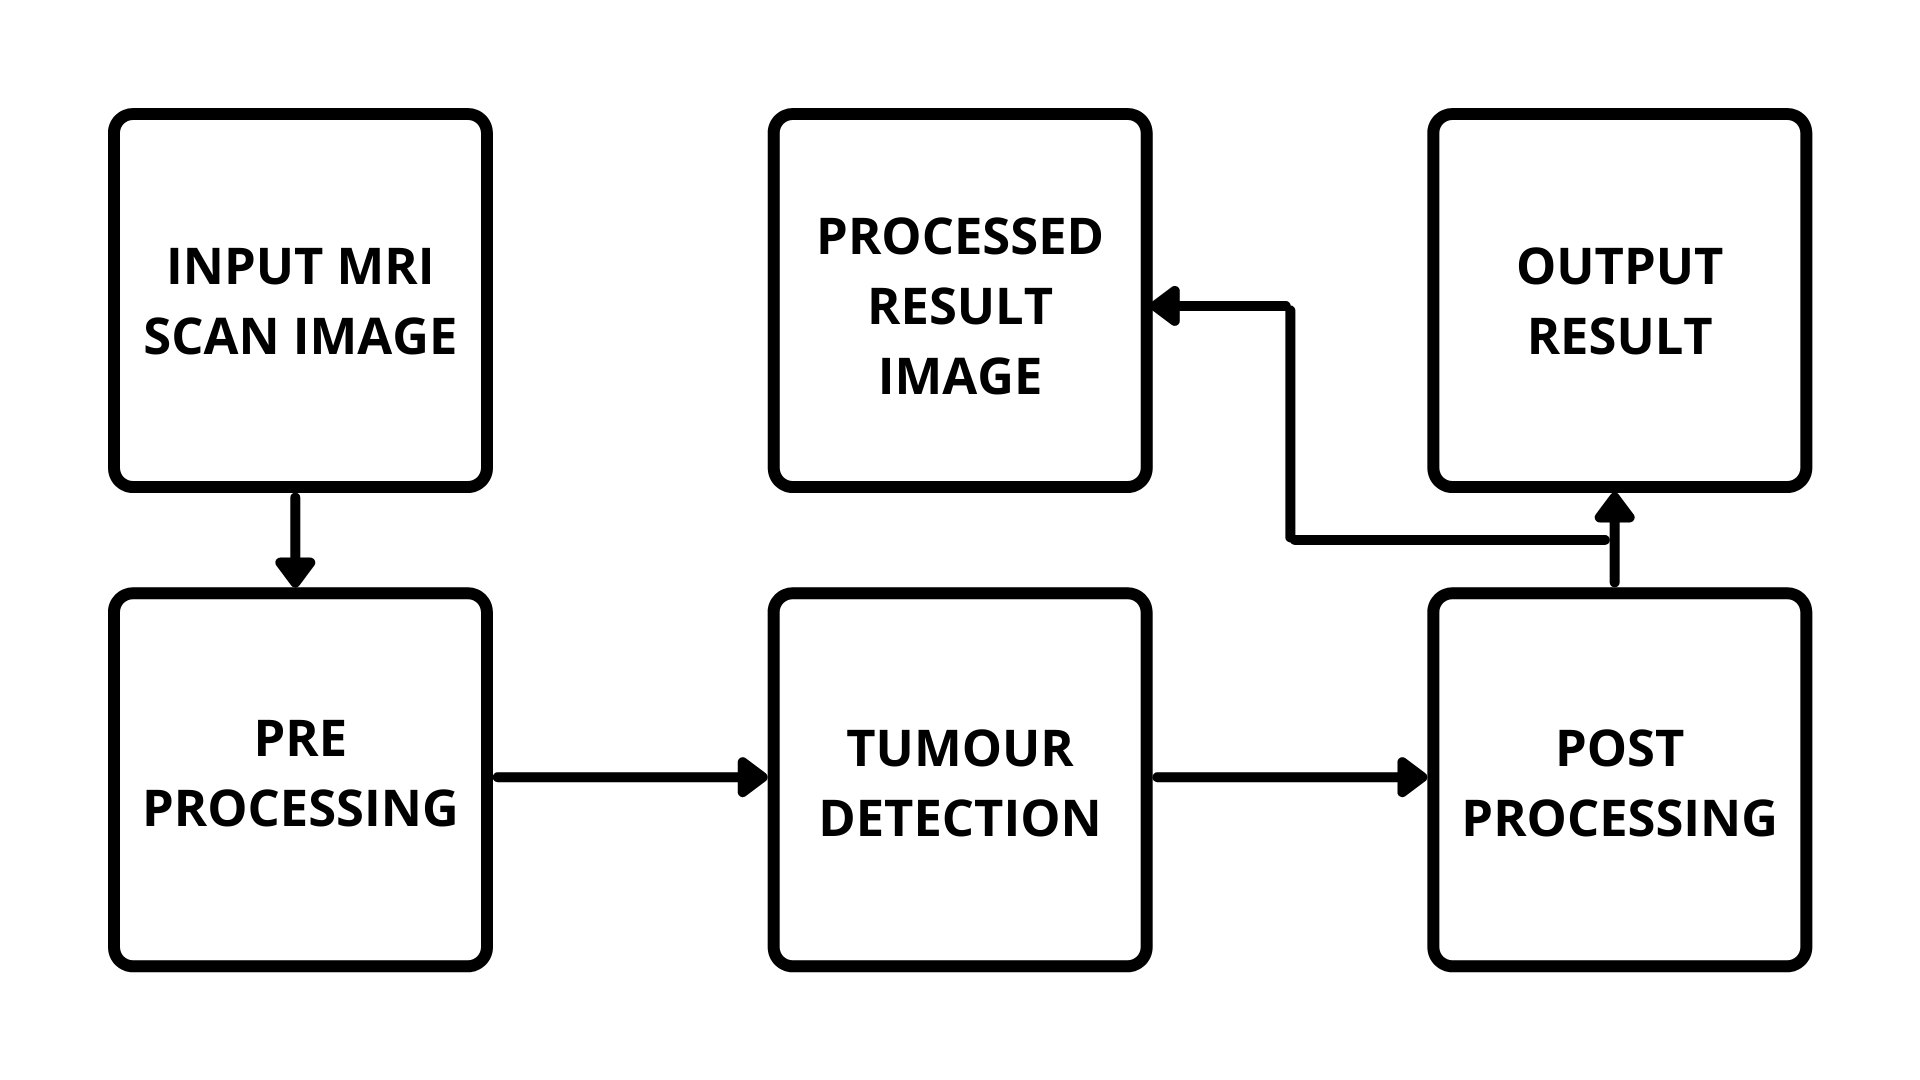
\includegraphics[scale=0.2]{Photos/blockdiagram.png}
\caption{Block Diagram} \label{fig:ishan}
\end{figure}
%%%%%%%%%%%%%%%%%%%%%%%%%%%%%%%%%%%%%%%%%%%%%%%%%%%%%%%%%%%%%
\section{Requirement analysis}
\subsection{Hardware Requirement}
The only hardware requirement for the project which has been observed till now are as follows:
\begin{itemize}
    \item An End device such as Laptop/PC(Both to train the model and for developing and accessing the web application)
\end{itemize}
%\subsection{Software Requirement}
%Explain about the appropriate Software Requirement with proper reasoning. (This is mandatory section)
\subsection{Modern Engineering Tools and Software Requirement}
{\textbf{a) Open Source Libraries / Softwares / Tools Requirement:}}
\begin{itemize}
    \item A python development environment : Any python environment is needed to train the model which will inturn detect the tumour. For our particular project we have opted for Kaggle Cloud Editor. For the mentioned below reasons:
        \begin{itemize}
            \item Higher computational power.
            \item Ease of importing data from datasets.
            \item Version control of code.
        \end{itemize}
        \begin{figure}[H]
        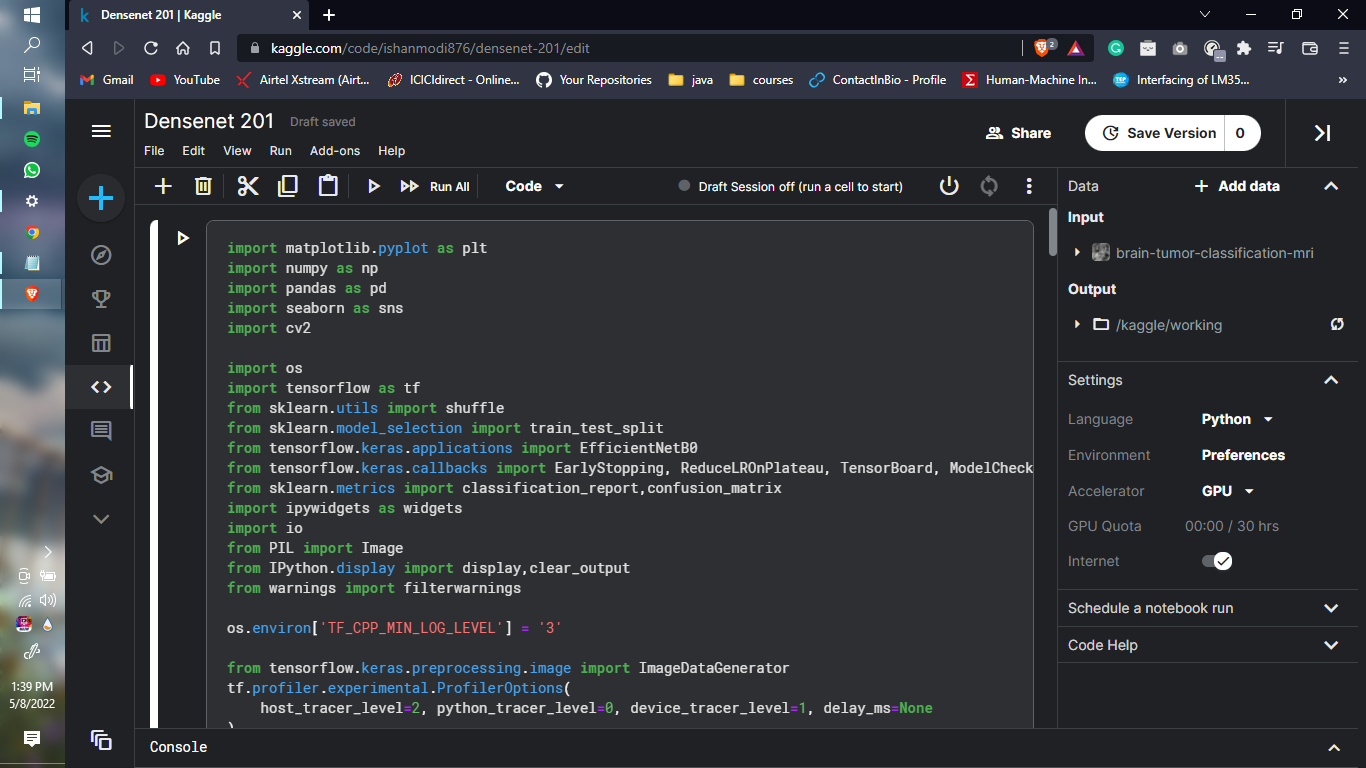
\includegraphics[scale=0.3]{Photos/Kaggle_Editor2.png}
        \caption{Kaggle Editor} \label{fig:ishan}
        \end{figure}
    \item Python Libraries : To implement the project, various libraries are needed to perform the required functionality that we desire. We need Python libraries both for the training of the model as well as to develop the web application. The libraries which have been used until now are as follows:
        % Please add the following required packages to your document preamble:
        % \usepackage{graphicx}
        % \usepackage[table,xcdraw]{xcolor}
        % If you use beamer only pass "xcolor=table" option, i.e. \documentclass[xcolor=table]{beamer}
        % Please add the following required packages to your document preamble:
% \usepackage{graphicx}
% \usepackage[table,xcdraw]{xcolor}
% If you use beamer only pass "xcolor=table" option, i.e. \documentclass[xcolor=table]{beamer}
        \begin{table}[h!]
        \caption{List of Python libraries used:}
        \label{tab:table1}
        \resizebox{\textwidth}{!}{%
        \begin{tabular}{|c|c|c|}
        \hline
        \rowcolor[HTML]{CBCEFB}  
\textbf{Library} & \textbf{Function}                                                                                                                                                                    & \textbf{Version(if applicable)} \\ \hline
OS               & \begin{tabular}[c]{@{}c@{}}Creating and removing a directory(folder),\\ fetching its contents, changing and identifying the current director.\end{tabular}                           & N/A                             \\ \hline
Keras            & \begin{tabular}[c]{@{}c@{}}Provide python interface for Neural Networks.\\ Also acts as an interface for Tensorflow Library.\\ Also used to define layers to the model.\end{tabular} & 2.6.0                           \\ \hline
Tensorflow       & \begin{tabular}[c]{@{}c@{}}Training and inference of deep neural networks.\\ Also used for establishing callbacks\end{tabular}                                                       & 2.6.1                           \\ \hline
Numpy            & Library for working with multi-dimensional arrays.                                                                                                                                   & 1.21.4                          \\ \hline
Pandas           & Data Manipulation and Analysis                                                                                                                                                       & 1.3.5                           \\ \hline
Matplotlib       & Data visualization and graphical plotting library                                                                                                                                    & 3.5.1                           \\ \hline
Sklearn          & \begin{tabular}[c]{@{}c@{}}Machine Learning library of Python.\\ Features various algorithms such as random forests, K-neighbours etc.\end{tabular}                                  & 0.23.2                          \\ \hline
Time             & Representing time in code                                                                                                                                                            & 3.7.0                           \\ \hline
Imutils          & Basic Image Processing                                                                                                                                                               & 0.5.4                           \\ \hline
Cv2              & Image Processing and computer vision                                                                                                                                                 & 4.5.4.60                        \\ \hline
Shutil           & Copy and Removal of files                                                                                                                                                            & 3.10.1                          \\ \hline
Seaborn          & Python Data Visualization library based on Matplotlib                                                                                                                                & 0.11.2                          \\ \hline
Ipywidgets       & Interactive HTML widgets for Jupyter and Ipython Console                                                                                                                             & 8.00rc0                         \\ \hline
\end{tabular}%
}
\end{table}
    \item LaTeX Editor : LaTeX is a high-quality typesetting system; it includes features designed for the production of technical and scientific documentation. LaTeX being a language system needs a system software to support it's functionality. For the project Papeeria has been used to write the project report.
    \item  \href{https://www.analyticsvidhya.com/blog/2021/06/build-web-app-instantly-for-machine-learning-using-streamlit/}{Streamlit Framework} : Streamlit is an open-source python framework for building web apps for Machine Learning and Data Science. We can instantly develop web apps and deploy them easily using Streamlit. Streamlit allows you to write an app the same way you write a python code. Streamlit makes it seamless to work on the interactive loop of coding and viewing results in the web app.
    %\begin{figure}[H]
    %    
\includegraphics[scale=0.001]{Photos/flask.png}
    %    \caption{Flask Web Framework} \label{fig:flask}
    %    \end{figure}
\end{itemize}
{\textbf{b) Proprietary Softwares / Libraries / Cloud Requirement:}}\\ 
Proprietary Software include both OS and software applications contained within it. The Proprietary Softwares which have been used in the duration of Phase-1 of the project are as follows:
\begin{itemize}
    \item Windows OS : Windows OS is the base Operating System, which has been used to develop the code base as well as to do the paper work.
    \item Microsoft Powerpoint : Microsoft Powerpoint is a proprietary software by Microsoft which has been used to make the presentations for the project as well as develop a proposed UI of the web application.
\end{itemize}
\subsection{Resources Requirement}
    \begin{itemize}
    \item Datasets : To train the model efficiently datasets are needed which contain the data(MRI scan images in our case). This data is fed to the model which then trains it to detect whether the MRI scan is tumorous or non-tumorous and further classify the tumorous images into 3 categories : Meningioma, Pituitary and Glioma. For the project one dataset has been utilized. The dataset contains 4 subfolders each containing images under four labels as follows : Pituitary, Meningioma, Glioma and Non-Tumorous . The Dataset is as follows:
        \begin{itemize}
            \item \href{https://www.kaggle.com/datasets/sartajbhuvaji/brain-tumor-classification-mri}{Brain Tumor Classification (MRI)} : \\
                Table (\ref{tab:Dataset}) gives an insight into the contents within the dataset: 
                % Please add the following required packages to your document preamble:
% \usepackage{multirow}
% \usepackage{graphicx}
% \usepackage[table,xcdraw]{xcolor}
% If you use beamer only pass "xcolor=table" option, i.e. \documentclass[xcolor=table]{beamer}
\begin{table}[h!]
                \caption{Contents of Brain MRI Images for Brain Tumor Detection Dataset}
                \label{tab:Dataset}
\begin{tabular}{c|c|c|}
\cline{2-3}
\multicolumn{1}{l|}{}                                                                                                        & \cellcolor[HTML]{CBCEFB}\textbf{Data Label} & \cellcolor[HTML]{CBCEFB}\textbf{No. Of Images} \\ \hline
\multicolumn{1}{|c|}{\cellcolor[HTML]{CBCEFB}}                                                                               & Glioma                                      & 100                                            \\ \cline{2-3} 
\multicolumn{1}{|c|}{\cellcolor[HTML]{CBCEFB}}                                                                               & Meningioma                                  & 115                                            \\ \cline{2-3} 
\multicolumn{1}{|c|}{\cellcolor[HTML]{CBCEFB}}                                                                               & No Tumour                                   & 105                                            \\ \cline{2-3} 
\multicolumn{1}{|c|}{\multirow{-4}{*}{\cellcolor[HTML]{CBCEFB}\textbf{\begin{tabular}[c]{@{}c@{}}Test\\ Set\end{tabular}}}}  & Pituitary                                   & 74                                             \\ \hline
\multicolumn{1}{|c|}{\cellcolor[HTML]{CBCEFB}}                                                                               & Glioma                                      & 826                                            \\ \cline{2-3} 
\multicolumn{1}{|c|}{\cellcolor[HTML]{CBCEFB}}                                                                               & Meningioma                                  & 822                                            \\ \cline{2-3} 
\multicolumn{1}{|c|}{\cellcolor[HTML]{CBCEFB}}                                                                               & No Tumour                                   & 395                                            \\ \cline{2-3} 
\multicolumn{1}{|c|}{\multirow{-4}{*}{\cellcolor[HTML]{CBCEFB}\textbf{\begin{tabular}[c]{@{}c@{}}Train\\ Set\end{tabular}}}} & Pituitary                                   & 827                                            \\ \hline
\end{tabular}%
\end{table} \\
Figure (\ref{fig:data_sample}) plots some sample images from the dataset.
\begin{figure}[H]
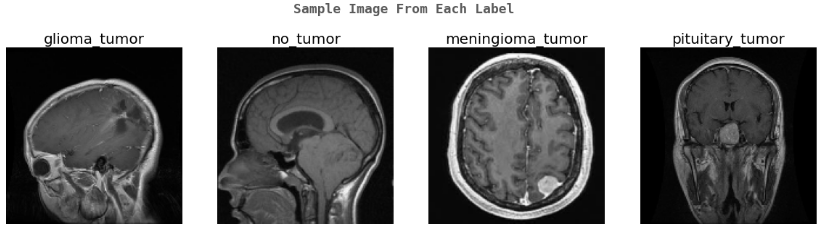
\includegraphics[scale=0.55]{Photos/dataset_sample1.PNG}
\caption{Sample Images from Dataset} \label{fig:data_sample}
\end{figure}
        \end{itemize}
        \item Graphical Images : Graphical Images are needed for the Web Application. This is purely a resource requirement for an end user product and is not needed for any core functionality of the system.
    \end{itemize}


\section{Impact analysis}
\subsection{Impact of project on society}
{\textbf{Positive Impact of project on society:}} 
\begin{itemize}
    \item Early detection of tumour can reduce the cost required to treat the tumour.
    \item Early detection can overall improve the lifespan of humans.
\end{itemize}
{\textbf{Negative Impact of project on society:}}
\begin{itemize}
    \item It has a risk of errors and wrong detection due to less training.
    \item It has a risk of not detecting Initial stages of tumour due to small size.
\end{itemize}
\subsection{Impact of project on environment }
{\textbf{Positive Impact of project on environment: }}
\begin{itemize}
    \item Less Bio Medical waste is generated due to early detection and treatment.
\end{itemize} 
{\textbf{Negative Impact of project on environment: }}
\begin{itemize}
    \item Bio Medical waste generated during treatment after the detection of tumour is done through this system, if not treated properly can pose environmental risks.
\end{itemize}

\section{Limitations}
\begin{itemize}
    \item Limited detection due to less datasets being used in training.
    \item Accuracy of Dataset is an important factor. Unverified datasets can lead to false results.
    \item The detection model in it's base form cannot provide accurate results on MRI captured using higher tesla MRI Machines.
\end{itemize}

\section{Professional ethical practices to be followed}
\begin{itemize}
    \item Giving credits wherever due.
    \item Keeping technical guidelines in mind.
    \item Following the norms of engineering Practices.
    \item Liabality for outcome caused by one’s actions or decisions.
\end{itemize}
